\section{Syntax of \lang{}}
\label{sec:syntax}

In this section, we introduce the syntax of \lang{}. A \lang{} program, as shown in the following block, essentially contains several parts,
\begin{bnf}
    \ntsym{program} ::=  (& \ntsym{typedef} | \ntsym{function} | \ntsym{automaton} | \ntsym{system})^*
\end{bnf}

% TODO: make it clear
\begin{enumerate}
    \item \emph{Typedef}s specifying alias for given types.
    \item \emph{Function}s defining customized functions that can be reused in other functions, automata and systems.
    \item \emph{Automaton}s defining automata through local variables and transitions.
    \item \emph{System}s declaring hierarchical structures of components and connections between the components. Both components and connections are described by automata.
\end{enumerate}

\subsection{Type System}
\label{subsec:typesystem}
\lang{} provides a rich-featured type system that supports various data types that are widely used in both formal modeling languages and programming languages.

\smalltitle{Primitive Types} Table \ref{table:primitivetypes} shows the primitive types supported by \lang{} including: \emph{ integers and bounded integers,  real numbers with arbitrary precision, boolean values, single characters (ASCII only) and finite enumerations}.

\begin{table}
    \caption{Primitive Data Types}
    \label{table:primitivetypes}
    \centering
    \begin{tabular}{lcr}
        \hline
        Name & Declaration & Term Example \T\B \\
        \hline
        \T 
        Integer & \texttt{int} & \texttt{-1,0,1} \\
        Bounded Integer\hspace{0.5cm} & \texttt{int lowerBound .. upperBound}\hspace{0.5cm} & \texttt{-1,0,1} \\
        Real & \texttt{real} & \texttt{0.1, 1E-3} \\
        Boolean & \texttt{bool} & \texttt{true, false} \\
        Character & \texttt{char} & \texttt{'a', 'b'} \\
        \B Enumeration & \texttt{enum {item$_1$, ..., item$_n$}} & \texttt{enumname.item} \\
        \hline
    \end{tabular}
\end{table}

\noindent\emph{Composite Types.} Composite types can be used to contruct complex data types from simpler ones. Several composite patterns are introduced as follows:

\begin{table}
    \caption{Composite Data Types (\texttt{T} denotes an arbitrary data type)}
    \centering
    \begin{tabular}{lr}
        \hline
        Name & Declaration \T\B \\
        \hline
        \T Tuple  & \texttt{T$_1$,...,T$_n$ }\\
        Union & \texttt{T$_1$|...|T$_n$ } \\
        Array & \texttt{T [length]}\\
        List & \texttt{T []} \\
        Map & \texttt{map [T$_{key}$] T$_{value}$} \\
        Struct\hspace{1cm} & \texttt{struct \{ field$_1$:T$_1$,..., field$_n$:T$_n$ \}} \\
        \B Initialized & \texttt{T$_{base}$ init term} \\
        \hline
    \end{tabular}
\end{table}

\begin{itemize}
    \item \emph{Tuple}. The \emph{tuple} operator `,' can be used to construct a finite tuple type with several base types.
    \item \emph{Union}. The \emph{union} operator `$|$' is designed to combine different types as a more complicated one. 
    \item \emph{Array} and \emph{List}. An \emph{array} $T[n]$ is a finite ordered collection containing exactly $n$ elements of type $T$. Moreover, a \emph{list} is an array of which the capacity is not specified, i.e. list is a dynamic array.
    \item \emph{Map}. A \emph{map }[$T_{key}$] $T_{val}$ is a dictionary that maps a key of type $T_{key}$ to a value of type $T_{val}$.
    \item \emph{Struct}. A \emph{struct }\{$field_1:T_1,\cdots,field_n:T_n$\} contains a finite number of fields, each has  a unique identifier $field_i$ and a particular type $T_i$.
    \item \emph{Initialized}. An initialized type is used to specify default value of a type $T_{base}$ with \texttt{term}.
\end{itemize}

\noindent\emph{Parameter Types}. A generalizable automaton or system that includes a template function or template component needs to be defined on many occasions. For example, a binary operator that support various operations ($+$,$\times$, etc.), or an encrypted communication system that supports different encryption algorithms. Parameter types make it possible to take functions, automata or systems as template parameters. \lang{} supports two parameter types: 
\begin{enumerate}
    \item \emph{An Interface}, denoted by \texttt{interface (port$_1$:T$_1$,$\cdots,$port$_n$:T$_n$)}, defines a parameter that could be any \emph{automaton} or \emph{system} with exactly the same interface (i.e. number, types and directions of the ports are a perfect match). Interfaces are only used in templates of \emph{system}s.
    % TODO: interfaces are not permitted in automata since automata do not support hierarchical structure
    \item \emph{A Function}, denoted by \texttt{func (arg$_1$:T$_1$,$\cdots, $arg$_n$:T$_n$):T}, defines a function that have the argument types $\texttt{T}_1,\cdots,\texttt{T}_n$ and result types \texttt{T}. Functions are permitted to appear in templates of \emph{other functions}, \emph{automata} and \emph{system}s.
\end{enumerate}

For simplicity, we use $Dom(T)$ to denote the value domain of type $T$, i.e. the set of all possible value of $T$.

\begin{example}[Types Used in a Queue] Queue is a well-known data structure being used in various message-oriented middlewares. In this example, we introduce some type declarations and local variables used in an automaton \texttt{Queue} defining the queue structure. As shown in the following code fragment, we declare a singleton enumeration \texttt{NULL}, which contains only one element \texttt{null}. The buffer of a queue is in turn formalized as an array of \texttt{T} or \texttt{NULL}, indicating that the elements in the queue can be either an assigned item or empty. The head and tail pointers are defined as two bounded integers.
\begin{lstlisting}
typedef enum {null} init null as NULL;
automaton <T:type,size:int> Queue(A:in T, B:out T) {
    variables {
        buf : ((T | NULL) init null) [size];
        phead, ptail : int 0 .. (size - 1) init 0;
    }
    ...
}
\end{lstlisting}
\label{exp:typeinqueue}
\end{example}

\subsection{Functions}
\label{subsec:functions}

Functions are used to encapsulate and reuse complex computation processes. In \lang{}, the notion of \emph{functions} is a bit different from most existing programming languages. \lang{} functions include no control statements at all but assignments, and have access only to its local variables and arguments. This design makes functions' behavior more predictable. In fact, the behavior of functions in \lang{} can be simplified into mathematical functions. 

The abstract syntax tree of functions is as follows.

\begin{bnf}
    \ntsym{funcDecl} ::= & \tsym{function} \ntsym{template}^? \ntsym{identifier} \tsym{(} \ntsym{arguments} \tsym{)} \tsym{\{} \\
    & (\tsym{variables} \tsym{\{} \ntsym{varDecl}^* \tsym{\}})^? \\
    & \tsym{statements} \tsym{\{} \ntsym{assignStmt}^* \ntsym{returnStmt} \tsym{\}} \\
    \ntsym{assignStmt} ::= & \ntsym{term} \tsym{:=} \ntsym{term} \\
    \ntsym{returnStmt} ::= & \tsym{return} \ntsym{term} \\
    \ntsym{varDecl} ::= & \ntsym{identifier} \tsym{:} \ntsym{type} (\tsym{init} \ntsym{term})^? 
\end{bnf}
Basically, a function definition includes the following parts.

\smalltitle{Template} A function may contain an optional template with a set of parameters. A parameter can be either a \emph{type} parameter (decorated by \texttt{type}) or a \emph{value} parameter (decorated by its type). Values of the parameters should be clearly specified during compilation. Once a parameter is declared, it can be referred in all the following language elements, e.g. parameter declarations, arguments, return types and statements.

\smalltitle{Name} An identifier that indicates the name of this function.

\smalltitle{Type} Type of a function is determined by its \emph{number and types of arguments}, together with \emph{the type of its return value.} 

\smalltitle{Body} Body of a function includes an optional set of local variables and a list of ordered statements that describe how the return value is computed. The statements always end by a \texttt{return} statement.

\begin{example}[Incline Operation on Queue Pointers] Incline operation of pointers are widely used in a \emph{round-robin} queue, where storage are reused circularly. The \texttt{next} function shows how pointers in such queues (denoted by a bounded integer) are inclined. 
    \label{exp:successor_function}
    \begin{lstlisting}
function <size:int> next(pcurr:int 0..(size-1)) : int 0..(size-1) {
    statements { return (pcurr + 1) % size; }
}
    \end{lstlisting}
\end{example}

\subsection{Automaton : The Basic Behavioral Unit}

Automata theory is widely used in formal verification. And its variations, finite-state machines for example, are also accepted by modeling tools like NI LabVIEW and Mathworks Simulink/Stateflow.

Here we introduce the notion of \emph{automaton} as the basic behavior unit. Compared with other variations, an \emph{automaton} in \lang{} contains local variables and typed ports that support complicated behavior and powerful communication. The abstract syntax tree of \emph{automaton} is as follows.

\begin{bnf}
    \ntsym{automaton} ::=& \tsym{automaton}\ntsym{template}^?\ntsym{identifier} \tsym{(} \ntsym{port}^* \tsym{)} \tsym{\{}\\
    & (\tsym{variables} \tsym{\{} \ntsym{varDecl}^* \tsym{\}})^? \\
    & \tsym{transitions} \tsym{\{} \ntsym{transition}^* \tsym{\}} \tsym{\}} \\
    \ntsym{port} ::=& \ntsym{identifier} \tsym{:} (\tsym{in}|\tsym{out}) \ntsym{type} \\
    \ntsym{transition} ::=& \ntsym{guardedStmt} | \tsym{group} \tsym{\{} \ntsym{guardedStmt}^* \tsym{\}}\\
    \ntsym{guardedStmt} ::=& \ntsym{term} \tsym{->} (\ntsym{stmt} | \tsym{\{} \ntsym{stmt}^* \tsym{\}}) \\
    \ntsym{stmt} ::=& \ntsym{term} \tsym{:=} \ntsym{term} | \tsym{sync} \ntsym{identifier}^+
\end{bnf}

\smalltitle{Template} Compared with templates in functions, templates in automata provide support for parameters of \emph{function type}.

\smalltitle{Name} The identifier of an automaton.

\smalltitle{Type} Type of an automaton is determined by the \emph{number} and \emph{type}s of its ports. Type of a port contains its \emph{direction} (either \texttt{in} or \texttt{out}) and its \emph{data type}. For example, a port $P$ that takes integer values as input is denoted by \texttt{P:in int}. To ensure the well-definedness of automata, ports are required to have an \emph{initialized} data type, e.g. \texttt{int 0..1 init 0} instead of \texttt{int 0..1}.

\smalltitle{Variables} Two classes of variables are used in an automaton definition. \emph{Local variables} are declared in the \emph{variables} segment, which can be referenced only in its owner automaton. \emph{Adjoint variables} are used to describe the status and value of ports.

Syntactically, adjoint variables are denoted as built-in fields of ports.
An arbitrary port $P$ has two boolean fields \texttt{P.reqRead} and \texttt{P.reqWrite} indicating whether there is any pending \emph{read} or \emph{write} requests on $P$, and a data field \texttt{P.value} indicating the current value of $P$. Adjoint variables are shared between automata to perform communications.
For an output port, the \texttt{reqRead} field is read-only and the \texttt{reqWrite} field is writable. Similarly, for an input port the \texttt{reqRead} field is writable but its \texttt{reqWrite} field is read-only. The \texttt{value} field can be assigned only when it belongs to an output port.

\smalltitle{Transitions}
In \lang{}, behavior of an automaton is described by a set of guarded transitions (groups), with no explicit concept of locations (actually locations can be easily encoded as local enumeration variables). A \emph{transition} (denoted by \emph{guard} \texttt{->} \emph{statements}) comprises two parts, a boolean term \emph{guard} that declares the activating condition of this transition, and a (sequence of) statement(s) describing how variables are updated when the transition is fired.

We have two types of statements supported in automata:
\begin{itemize}
    \item \emph{Assignment Statement} (\texttt{var$_1$,...,var$_n$ := term$_1$,...,term$_n$}). Assignment statements update variables with new values where only local variables and writable adjoint variables are assignable.
    \item \emph{Synchronizing Statement} (\texttt{sync port$_1$,...,port$_n$}). Synchronizing statements are used as synchronizing \emph{flag}s when joining multiple automata. In a synchronizing statement, the order of ports being synchronized is arbitrary. 
\end{itemize}

% TODO: why not so simple as for ?
With the introduction of adjoint variables, synchronizing transitions in automata joining is not so simple as in traditional automata models where all variables are local. Informally speaking, the synchronizing statements are used to properly schedule the assignment operations in different automata.

Synchronizing statements are also important flags to distinguish between external transitions and internal transitions. A transition is called \emph{external} iff. it synchronizes with its environment through some ports, or \emph{internal} otherwise. Literally, all transitions, where synchronizing statements are involved, are \emph{external} transitions. In such transitions, the following rules should be strictly followed.

\begin{enumerate}
    \item Any assignment statements including reference to an input port should be placed after its corresponding synchronizing statement.
    \item Any assignment statements to an output port should be placed before its corresponding synchronizing statement.
\end{enumerate}


We use $g\rightarrow S$ to denote a transition, where $g$ is the guard formula and $S=[s_1,\cdots,s_n]$ is a sequence of statements. 

Transitions in \lang{} automata are organized with \emph{priority}. A transition has higher priority than all the other following ones. When multiple transitions are activated simultaneously by the environment, the one with highest priority will be fired first. 
% Formally speaking, suppose $g_1\rightarrow S_1,\cdots,g_n\rightarrow S_n$ is a list of transitions with priority, we could use an equivalent form to rewrite them as the followings, where priority is not necessary any more.
% \[
%     g_1\rightarrow S_1, \lnot g_1\land g_2\rightarrow S_2,\cdots,\lnot g_1\land \lnot g_2\land\cdots\land \lnot g_{n-1} \land g_n\rightarrow S_n
% \]

\begin{example}[Transitions in Queue] For a queue, we use internal transitions to capture the modifications corresponding to the changes of its environment. For example, the automaton \texttt{Queue}  tries to:
\begin{enumerate}
    \item Read data from its input port $A$ by setting \texttt{A.reqRead} to \emph{true} when the buffer isn't full.
    \item Write the earliest existing buffered data to its output port $B$ when the buffer is not empty. 
\end{enumerate}
External transitions, on the other hand, mainly show the implementation details for the enqueue and dequeue operations.
\begin{lstlisting}
// internal transitions
!A.reqRead && (buf[phead] == null) -> A.reqRead := true;
A.reqRead && (buf[phead] != null) -> A.reqRead := false;
!B.reqWrite && (buf[ptail] != null) -> B.reqWrite := true;
B.reqWrite && (buf[ptail] == null) -> B.reqWrite := false;

// enqueue operation (as an external transition)
(A.reqRead && A.reqWrite) -> {
    sync A; buf[phead] := A.value; phead := next(phead);
}
// dequeue operation (as an external transition)
(B.reqRead && B.reqWrite) -> {
    B.value := buf[ptail]; ptail := next(ptail); sync B;
}
\end{lstlisting}
\label{exp:trans_queue}
\end{example}

If all transitions are organzied with priority, the automata would be fully deterministic. However, in some cases non-determinism is still more than necessary. Consequently, we introduce the notion of \emph{transition group} to capture non-deterministic behavior. A transition group $t_G$ is formalized as a finite set of guarded transitions
$t_G=\{t_1,\cdots, t_n\}$ where $t_i=g_i\rightarrow S_i$ is a single transition with guard $g_i$ and a sequence of statements $S_i$.

Transitions encapsulated in a \texttt{group} are not ruled by priority. Instead, the group itself is literally ordered w.r.t. other groups and single transitions (basically, we can take all single transitions as a singleton transition group).

\begin{example}[Another Queue Implementation] In Example \ref{exp:trans_queue}, when both \emph{enqueue} and \emph{dequeue} operations are activated, \emph{enqueue} will always be fired first. Such a queue may get stuff up immediately when requests start accumulating, and in turn lead to excessive memory usage. With the help of transition groups, here we show another non-deterministic implementation which solves this problem.
\begin{lstlisting}
group {
    // enqueue operation (as an external transition)
    (A.reqRead && A.reqWrite) -> {
        sync A; buf[phead] := A.value; phead := next(phead);
    }
    // dequeue operation (as an external transition)
    (B.reqRead && B.reqWrite) -> {
        B.value := buf[ptail]; ptail := next(ptail); sync B;
    }
}
\end{lstlisting}
In the above code fragment, the two external transitions are encapsulated together as a transition group. Consequently, firing of the dequeue operation doesn't rely on deactivation of the enqueue operation.
\label{exp:transgroup_queue}
\end{example}


We use a 3-tuple $A=\langle Ports, Vars, Trans_G \rangle$ to represent an automaton in \lang{}, where $Ports$ is a set of ports, $Vars$ is a set of local variables (the set of adjoint variables are denoted by $Adj(A)$, which can be obtained from $Ports$ directly) and $Trans_G=[t_{G_1},\cdots,t_{G_n}]$ is a sequence of transition groups, where all single transitions are encapsulated as singleton transition groups.

\subsection{System : The Composition Approach}
\label{subsec:system}

Theoretically, automata and their product is capable to model various classical applications. However, modeling complex systems through a mess of transitions and tons of local variables could become a real disaster.

As mentioned before, \lang{} is designed to help the programmers, even nonprofessionals, to enjoy the convenience of formal tools. And that is exactly the reason why we introduce the notion of \emph{system} in the language. Basically, a \emph{system} is the textural representation of a hierarchical diagram where automata and smaller systems are organized as different roles (\emph{component}s or 
\emph{connection}s). 

% Hierarchical diagrams have already been used in various modeling tools (for example, SCADE \cite{AbdullaISoLA2006,BerryScp1992}, Simulink \cite{hahn2016essentialsimulink} and LabVIEW \cite{labview}). However, in most tools, connections are simply synchronous link that seal two ports together. Inspired by the connectors in Reo, \lang{} to declare an automaton as a connection, which lead to more powerful and intuitive diagrams. 

\begin{example}[A Message-Oriented Middleware]
    A simple diagram of a message-oriented middleware \cite{CurryMfc2004} is provided in Fig. \ref{fig:diagram}, where a queue works as a connector to coordinate the behavior of different components (message producers and consumers).
\end{example}

\begin{figure}
    \centering
    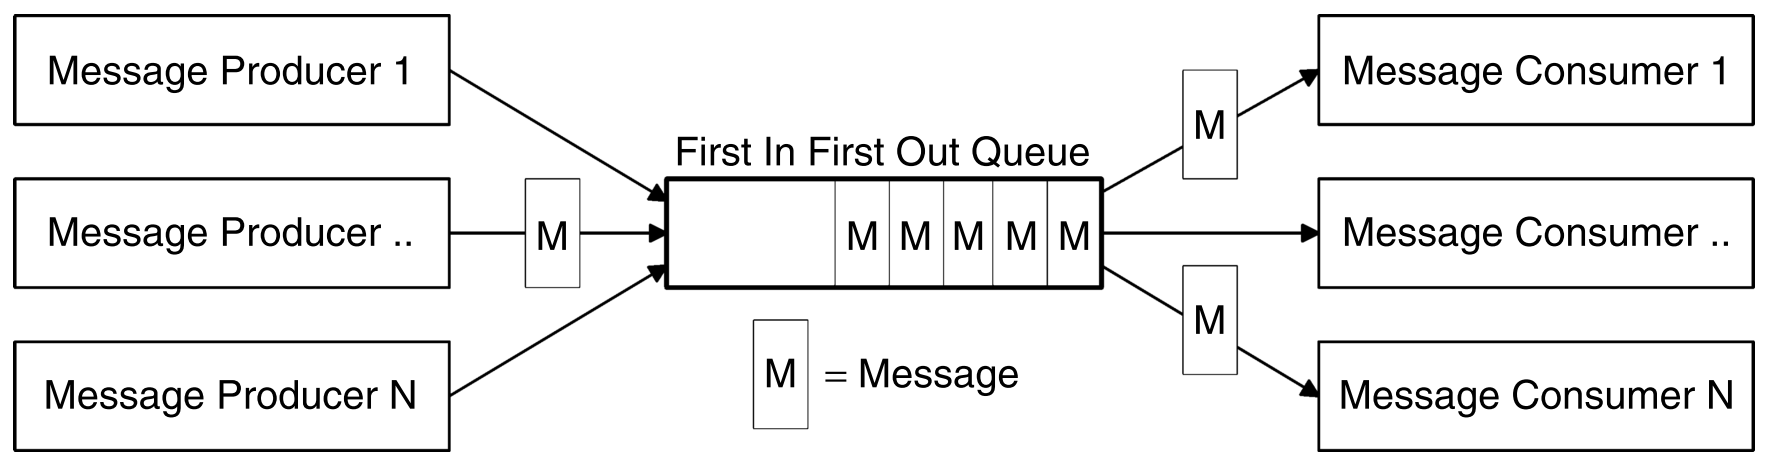
\includegraphics[width=.8\textwidth]{images/middleware_queue.png}
    \caption{A Senerio where Queue is used as Message-Oriented Middleware}
    \label{fig:diagram}
\end{figure}

The abstract syntax tree of \emph{system}s is as follows:
\begin{bnf}
    \ntsym{system} ::= & \tsym{system} \ntsym{template}^?\ntsym{identifier} \tsym{(} \ntsym{port}^* \tsym{)} \tsym{\{}\\
    & (\tsym{internals} \ntsym{identifier}^+)^? \\
    & (\tsym{components} \tsym{\{} \ntsym{componentDecl}^* \tsym{\}})^? \\
    & \tsym{connections} \tsym{\{} \ntsym{connectionDecl}^* \tsym{\}} \tsym{\}}\\
    \ntsym{componentDecl} ::= & \ntsym{identifier}^+ \tsym{:} \ntsym{systemType} \\
    \ntsym{connectionDecl} ::= & \ntsym{systemType} \ntsym{params} \tsym{(} \ntsym{portName}^+ \tsym{)}
\end{bnf}

% The \emph{type} of a system (i.e. its template, name, and ports) shares exactly the same form and meaning with \emph{type} of an automaton. This also suggests that system is NOT a special semantics unit, but simply an compositional approach to pile up automata.
% We declare a system with its template, name and type, then it is implemented by an optional set of \emph{internal node}s, an optional set of \emph{component}s and a set of \emph{connection}s.

\smalltitle{Template} In templates of systems, all the parameter types being supported include: \emph{a)} parameters of abstract type \texttt{type}, \emph{b)} parameters of primitive types and composite types, and \emph{c)} interfaces and functions.

\smalltitle{Name and Type} Exactly the same as \emph{name} and \emph{type} of an automaton.

\smalltitle{Components} In \texttt{components} segments, we can declare any entity of an \emph{interface type} as components, e.g. an automaton, a system, or a parameter of interface type. 
Ports of a component can be referenced by \texttt{identifier.portName} once declared.

\smalltitle{Connections} Connections, e.g. the arrows in Fig. \ref{fig:diagram}, are used to connect \emph{a) the ports of the system itself, b) the ports of its components, and c) the internal nodes}. We declare the connections in \texttt{connections} segments.
Both components and connections are supposed to run as automata in parallel.

\smalltitle{Internals} In certain cases, we need to combine multiple connections to perform more complex coordination behavior. Internal nodes, as declared in \texttt{internals} segments, are untyped identifiers which are capable to weld two ports with consistent data-flow direction. In other words, an internal node receives data from one port and sends it to another simultaneously.

% Essentially, data flow in an internal node should always follow the same direction, i.e. an internal node doesn't collect or generate any data, it only receives from one end and forward it simultaneously. The direction, together with the type of an internal node, should be determined when being compiled.

A system is denoted by a 4-tuple
$S=\langle Ports, Entities, Internals, Links\rangle$ where $Ports$ is a set of ports, $Entities$ is a set of automata or systems (including both components and connections), $Internals$ is a set of internal nodes and $Links$ is a set of pairs, where each element of such a pair is either a port or an internal node. A link $\langle p_1,p_2\rangle$ suggests that $p_1$ and $p_2$ are linked together. A well-defined system satisfies the following assumptions:

% TODO:
\begin{enumerate}
    \item $\forall \langle p_1,p_2\rangle \in Links$, data transfer from $p_1$ to $p_2$. For example, if $p_1\in Ports$ is an input port, $p_2$ could be
    \begin{itemize}
        \item an output port of the system ($p_2\in Ports$), 
        \item an input port of some automaton $A_i\in Automata$ ($p_2\in A_i.Ports$), or
        \item an internal node ($p_2\in Internals$).
    \end{itemize}
    \item $\forall n\in Internals,\exists!p_1,p_2$, s.t. $\langle p_1,n\rangle ,\langle n,p_2\rangle\in Links$ and $p_1,p_2$ have the same data type.
\end{enumerate}

\begin{example}[\lang{} Model of the System in Fig. \ref{fig:diagram}] In Fig. \ref{fig:diagram}, a simple scenario is presented where a queue is used as a message-oriented middleware. To model this scenario, we need two automata \emph{Producer} and \emph{Consumer} (details are omitted due to space limit, and can be found at \cite{medmodels}) that produce or consume messages of type \emph{T}.
\begin{lstlisting}
automaton <T:type> Producer (OUT: out T) { ... }
automaton <T:type> Consumer (IN: in T) { ... }

system <T:type> middleware_in_use () {
    components {
        producer_1, producer_2, producer_3 : Producer<T>;
        consumer_1, consumer_2, consumer_3 : Consumer<T>;
    }
    internals  M1, M2 ;
    connections {
        Merger<T>(producer_1.OUT, producer_2.OUT, producer_3.OUT, M1);
        Queue<T>(M1, M2);
        Replicator<T>(M2, consumer_1.IN, consumer_2.IN, consumer_3.IN);
    }
}
\end{lstlisting}
\label{exp:middleware_system}
\end{example}